\begin{tikzpicture}
    \node[anchor=south west,inner sep=0] (cdssimage) at (0,0) {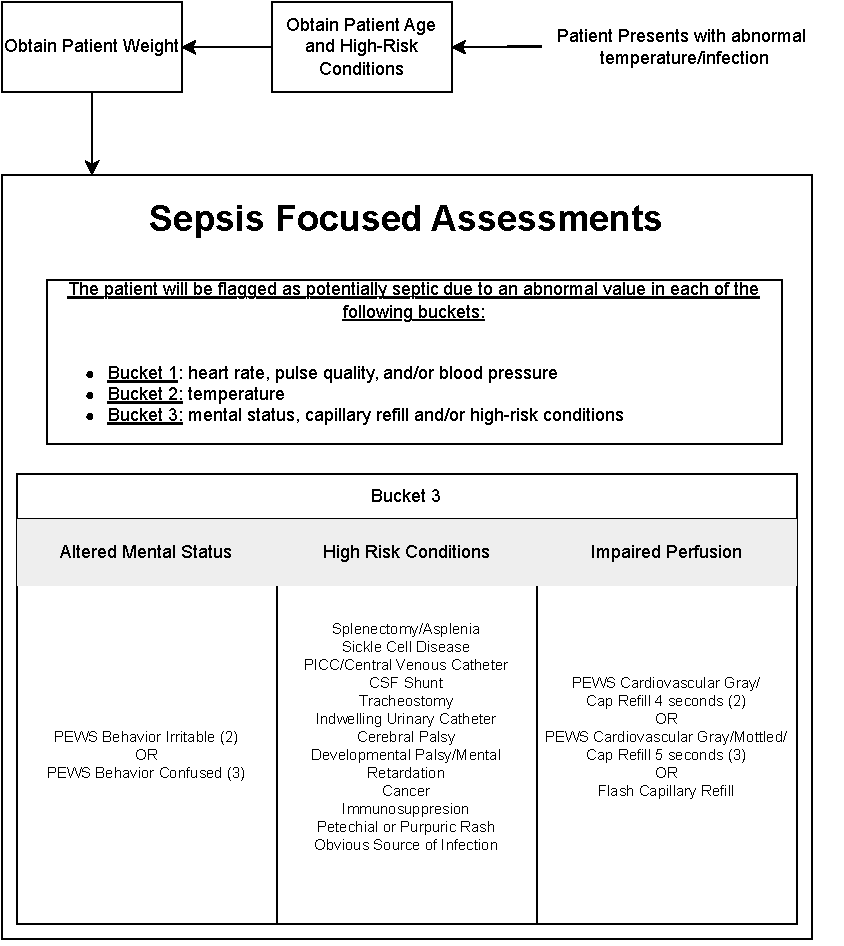
\includegraphics[width=0.9\textwidth]{sepsis-screening-osf}};
    \begin{scope}[x={(cdssimage.south east)},y={(cdssimage.north west)}]
        %\draw[help lines,xstep=.1,ystep=.1] (0,0) grid (1,1);
        %\foreach \x in {0,1,...,9} { \node [anchor=north] at (\x/10,0) {0.\x}; }
        %\foreach \y in {0,1,...,9} { \node [anchor=east] at (0,\y/10) {0.\y}; }
        \draw<2>[red] (0.0001,0.9) rectangle (0.22,0.999);
        \draw<3>[red] (0.0001,0.0) rectangle (0.965,0.82);
    \end{scope}
\end{tikzpicture}
